% !TEX root = ../notes_unsupervisedlearning.tex
% Chapter 6: Variational Inference and VAEs




% TODO: Add an image at why deep learning which shows the different semantic levels of the representation, 
% and how they compose to capture complex structure with fewer parameters than a shallow network.
% also maybe add a little break out into loss landscape engineering (numeric?)
% 
%
%
%
%%%%%%%%%%%%%%%%%%%%%%%%%%%%%%%%%%%%%%%%%%%%%%%%%%%%%%%%%%%%%%%%%%%%%%

\chapter{Variational Inference}\index{VAE}\index{Variational Autoencoder}\index{ELBO}
\newthought{embeddings and latent feature spaces.}

% ==============================================================================================
% BLOCK 1: INTRODUCTION
% ==============================================================================================

\section{The Why}\index{variational inference}\index{latent variable model}

\marginnote{\newthought{Plato's cave allegory}\cite{Plato380BC} describes prisoners who see only shadows on a wall,
never the objects that cast them. The shadows are high dimensional and entangled; the true forms behind them are few and independent. Dimensionality reduction, as we have seen, tries to recover those forms from the shadows. This chapter asks two follow-up questions: can we organise the recovered forms into a structured, reusable feature space, and once we have that space, can we cast new, plausible shadows we have never observed?}

\newthought{The central problem of unsupervised learning} is representation learning\index{representation learning}:
finding a mapping from raw observations to a latent feature space in which the underlying
factors of variation become explicit.
Bengio, Courville, and Vincent\cite{Bengio2013} argue that the
quality of a representation determines the success of any downstream task, and that a good
representation disentangles the factors that explain the data.

\newthought{PCA gave us a first answer:} project onto the directions of maximum variance.
But PCA is linear; it cannot recover structure that lies on a curved manifold.
What we lack is a parametric encoder
that can be applied to new, unseen data or reused as a feature extractor on nonlinear feature spaces.

\newthought{Autoencoders}\index{autoencoder} close that gap.
Hinton and Salakhutdinov\cite{Hinton2006} showed that a neural network can learn a nonlinear,
low-dimensional embedding $z$ from which a second network reconstructs $\hat{x}$,
outperforming PCA on complex data.
The encoder $\theta_E\colon \mathbb{R}^d \to \mathbb{R}^k$ and the decoder
$\theta_D\colon \mathbb{R}^k \to \mathbb{R}^d$ are trained jointly to minimise
reconstruction error $\|x - \theta_D(\theta_E(x))\|^2$.
The bottleneck forces the network to discover a compact representation.

\begin{figure}
\centering
\begin{tikzpicture}[
    every node/.style={font=\small, align=center},
    block/.style={rectangle, draw=black, thick, rounded corners=2pt,
                  minimum width=2.4cm, minimum height=0.7cm, inner sep=4pt},
    arr/.style={-{Triangle[length=4pt, width=4pt, fill=black!70]}, thick, black!70},
]
    \node[block] (input) {$x \in \mathbb{R}^d$};
    \node[font=\footnotesize, anchor=west, text width=1.6cm, align=left]
        at ([xshift=4pt]input.east) {\textsc{raw\\observation}};

    \node[block, below=24pt of input, fill=black!8] (hidden) {$z \in \mathbb{R}^k$};
    \node[font=\footnotesize, anchor=west, text width=1.6cm, align=left]
        at ([xshift=4pt]hidden.east) {\textsc{learned\\representation}};

    \node[block, below=24pt of hidden] (output) {$\hat{x} \in \mathbb{R}^d$};
    \node[font=\footnotesize, anchor=west, text width=1.6cm, align=left]
        at ([xshift=4pt]output.east) {\textsc{reconstruction}};

    \draw[arr] (input.south) -- node[left, font=\tiny, xshift=-1pt] {$\theta_E$} (hidden.north);
    \draw[arr] (hidden.south) -- node[left, font=\tiny, xshift=-1pt] {$\theta_D$} (output.north);
\end{tikzpicture}
\caption{Autoencoder architecture. The encoder $\theta_E$ maps the input to a low-dimensional representation; the decoder $\theta_D$ reconstructs the input from it. The bottleneck forces the network to discover a compact latent feature space.}
\label{fig:autoencoder_architecture}
\end{figure}


\newthought{Structure requires a probabilistic formulation.}

\marginnote{\newthought{A prior} is the distribution we assume over the latent space before seeing any data.}

If we replace the deterministic bottleneck with a distribution,
and regularise that distribution toward a known prior,
the latent space becomes smooth and complete:
every region maps to a plausible output, and nearby embeddings correspond to similar inputs.
Kingma and Welling\cite{KingmaWelling2014} formalised this idea as the Variational Autoencoder\index{VAE},
deriving a principled training objective from variational inference that balances
faithful reconstruction against latent space regularity.

\newthought{All of this must happen without labels.}
Supervised learning can organise a feature space by asking ``which class does this input belong to?'' and adjusting representations until the answer is easy to read off.
An unsupervised model has no such signal.
Instead, it must derive structure from the data alone, using two complementary pressures: the requirement to reconstruct the input faithfully, and the requirement to keep the latent space close to a known prior.
Reconstruction forces the embedding to retain information; the prior forces the embedding to be organised.
Neither pressure requires a human to annotate a single example.

\newthought{In order to move from reconstruction-only embeddings to well-organised latent feature spaces} we have good reason to find ways to,
\begin{itemize}
    \item formulate a learning objective that rewards both faithful reconstruction and a smooth, regular latent space.
    \item train a model that outputs distributions rather than points, so that the latent space has no undefined gaps.
    \item control how much structure the latent space carries, and understand how that choice affects the quality of the learned representation.
\end{itemize}








% ---------------------------------------------------------------------------
\newpage
\subsection{Hands-On Experience}

\newthought{Form groups of two:} an encoder and a decoder.
Prepare five digit cards showing \textbf{0}, \textbf{1}, \textbf{3}, \textbf{7}, and \textbf{8}.
Shuffle them face down on the table.

\marginnote{\newthought{Scoring.}
After the decoder guesses, flip the card.
Correct digit $= 0$, wrong digit $= 1$.
Sum over all rounds: that is your reconstruction loss.}

\newthought{Step 1: Design your features.}
The encoder picks two properties of digit shapes and writes them down.
These are your two latent features $z^{(1)}$ and $z^{(2)}$.
For example: $z^{(1)} =$ ``number of closed loops'' (0 has one, 8 has two, 1 has none)
and $z^{(2)} =$ ``has a straight vertical stroke'' (1 yes, 7 yes, 0 no); make sure to come up with your own
The decoder does not see these definitions.

\newthought{Step 2: Play.}
Each round, the encoder flips one card, looks at the digit, and writes two numbers
$(z^{(1)}, z^{(2)})$ on a slip of paper.
The decoder receives only the slip and guesses which digit it is.
Then reveal the card.
The decoder now knows: ``the embedding $(1, 0)$ meant the digit 3.''
Round by round, the decoder builds a mental map of what the embeddings mean.
When all five cards are done, shuffle and keep going.

\newthought{Step 3: Observe.}
In early rounds, the decoder guesses blindly.
With each reveal, the decoder learns what the embeddings mean.
At some point the reconstruction loss drops to zero: the decoder has learned
the encoder's representation from examples alone.

\newthought{Step 4: Record and compare.}
Plot your five embeddings in the coordinate system below.

\begin{figure}
\centering
\begin{tikzpicture}
    \begin{axis}[
        xlabel={$z^{(1)}$},
        ylabel={$z^{(2)}$},
        xmin=-3, xmax=3,
        ymin=-3, ymax=3,
        width=0.5\textwidth,
        height=0.5\textwidth,
        axis line style={draw=none},
        tick style={black, thick},
        xtick={-2,-1,0,1,2},
        ytick={-2,-1,0,1,2},
        xticklabel style={font=\small},
        yticklabel style={font=\small},
        tick align=outside,
        tick pos=left,
    ]
    \end{axis}
\end{tikzpicture}
\caption{Your latent space. Plot the five digit embeddings at the coordinates $(z^{(1)}, z^{(2)})$ your encoder chose.}
\label{fig:handson_latent}
\end{figure}

\marginnote{
\begin{itemize}
    \item How many rounds did the decoder need before reconstructions became reliable?
    \item Which digits did the decoder confuse most often? What does that tell you about your feature choice?
\end{itemize}}

\newthought{Step 5: Swap decoders.}
Find another group. Send your decoder to them, take theirs.
Play one more pass with the swapped decoder.

The swapped decoder has learned a different codebook: in their group, $(1, 0)$ might have meant ``7,''
in yours it means ``3.'' The reconstruction loss jumps back up.
The problem is not that either representation is wrong; both worked within their own group.
The problem is that nothing forced the two groups to organise their embeddings the same way.


\newthought{Step 6: Shrink the bottleneck.}
Drop to a single latent feature $z^{(1)}$.
The encoder must pick the one property that matters most; the decoder has only one number to work with.
Play a full pass and record the new reconstruction loss.

\newthought{Step 7: Discretise.}
Go back to two features, but restrict each to binary values (0 or 1).
The encoder can no longer spread digits across a continuous range and must find features that cleanly partition the digit set with just two bits.

\newthought{Step 8: Add digits.}
Keep two binary features, but add the cards \textbf{2}, \textbf{4}, \textbf{5}, and \textbf{9}.
A representation that separated five digits may collapse when it must also distinguish eight.
But the extra classes also expose ad hoc feature choices: properties that happened to work for a small set get overwhelmed, and the encoder is pressured toward genuinely structural features (loops, strokes, intersections) that scale.

\newthought{Step 9: Swap decoders again.}
Find a different group than in Step~5. Exchange decoders and play one pass with the expanded digit set.
Compare the reconstruction loss to the Step~5 swap: did the stress tests in Steps 6 to 8 push both groups toward more compatible representations.
\marginnote{After each decoder swap, collect the chosen latent features from all groups on the board. Are the feature sets converging across the room? Which features survived the stress tests and which were abandoned?}

\newthought{Each step hurts reconstruction} but forces the encoder to find features
that generalise across inputs rather than overfit to a narrow set.
This tension between reconstruction fidelity and generalisation through 
compression or broader coverage
is exactly the trade-off that the VAE formalises.
And a trade-off you know from supervised learning as well, overfitting versus generalization.

\marginnote{\newthought{Two objectives, one game.}
Steps 2 to 4 trained the reconstruction part: the decoder learned to recover digits from embeddings.
Steps 5 and 9 exposed the missing regularisation: without a shared convention for what the embeddings mean,
a new decoder cannot read them.
Steps 6 to 8 showed that compression and broader coverage force better features.
A VAE adds exactly this second pressure: it forces every encoder to arrange its embeddings
according to a shared prior, so that any decoder can use them.}

\newthought{This is the representation learning problem.}
Every choice of features defines a different geometry: different neighbours, different distances.
Within one encoder-decoder pair, reconstruction works.
Across pairs, the embeddings are incompatible.

\newthought{The fundamental question} is: can we add a shared convention to the latent space,
so that the embeddings are not only good for reconstruction but also follow a common structure
that any decoder could interpret?




\newthought{The Learning Objectives} of this lecture:
\begin{itemize}
    \item The Autoencoder Training Cycle. Architecture, forward pass, reconstruction loss, backpropagation, and what the bottleneck forces the network to learn.
    \item From Autoencoders to VAEs. Why reconstruction alone leaves the latent space unstructured, and what a probabilistic formulation buys us.
    \item The Evidence Lower Bound. The training objective that balances faithful reconstruction against latent space regularity.
    \item The Reparameterisation Trick. How to backpropagate through a stochastic sampling step.
    \item VAE Training and Bottleneck Design. Practical choices that shape the latent space: loss functions, latent dimensionality, and numerical stability.
    \item Exploring the Latent Space. Interpolation and generation as tests of representation quality.
    \item VAE Variants. How they each change one structural assumption.
    \item Feature Extraction, Transfer, and Distillation. Using the trained encoder as a backbone for downstream tasks.
\end{itemize}







% ==============================================================================================
% BLOCK 2: MAIN THEORY
% ==============================================================================================

% ---------------------------------------------------------------------------
\newpage

\section{The Autoencoder}\index{autoencoder}\index{reconstruction loss}

Follows the notion of a bottleneck architecture: an encoder that compresses the input into a low-dimensional embedding, 
and a decoder that reconstructs the input from that embedding. Due to the bottleneck, the encoder must learn to extract the most salient features of the input, 
and the decoder must learn to use those features to reconstruct the input as losslessly as possible.

\begin{figure}
    \centering
    \begin{tikzpicture}[
        every node/.style={font=\small, align=center},
        block/.style={rectangle, draw=black, thick, rounded corners=2pt,
                      minimum width=2.4cm, minimum height=0.7cm, inner sep=4pt},
        arr/.style={-{Triangle[length=4pt, width=4pt, fill=black!70]}, thick, black!70},
        gradarr/.style={-{Triangle[length=4pt, width=4pt, fill=black!30]}, thick, black!30, densely dashed},
    ]
        \node[block] (input) {$x \in \mathbb{R}^d$};
        \node[block, below=24pt of input, fill=black!8] (hidden) {$z \in \mathbb{R}^k$};
        \node[block, below=24pt of hidden] (output) {$\hat{x} \in \mathbb{R}^d$};
        \node[font=\small, below=18pt of output] (loss) {$\mathcal{L} = \|x - \hat{x}\|^2$};
    
        % Forward arrows
        \draw[arr] (input.south) -- node[left, font=\tiny, xshift=-1pt] {$\theta_E$} (hidden.north);
        \draw[arr] (hidden.south) -- node[left, font=\tiny, xshift=-1pt] {$\theta_D$} (output.north);
        \draw[arr] (output.south) -- (loss.north);
    
        % Gradient arrows (right side, dashed)
        \draw[gradarr] ([xshift=10pt]loss.north) -- ([xshift=10pt]output.south);
        \draw[gradarr] ([xshift=10pt]output.north) -- ([xshift=10pt]hidden.south);
        \draw[gradarr] ([xshift=10pt]hidden.north) -- ([xshift=10pt]input.south);
    \end{tikzpicture}
    \caption{Autoencoder training cycle. Solid arrows: forward pass ($x \to z \to \hat{x} \to \mathcal{L}$). Dashed arrows: gradient flow back through decoder and encoder.}
    \label{fig:ae_training_cycle}
    \end{figure}

    \marginnote{\newthought{Notation.} $\theta_E$ denotes the encoder; $\theta_D$ denotes the decoder. Both are neural networks trained jointly.}


\newthought{The encoder} $\theta_E\colon \mathbb{R}^d \to \mathbb{R}^k$ compresses a $d$-dimensional input $x$ into a $k$-dimensional embedding $z$, with $k \ll d$.

\newthought{The decoder} $\theta_D\colon \mathbb{R}^k \to \mathbb{R}^d$ takes $z$ and attempts to reconstruct the original input as $\hat{x}$.

\marginnote{\newthought{Backpropagation} is the backbone of supervised learning, and it applies here unchanged.
The loss $\mathcal{L}$ depends on $\theta_D$ (through $\hat{x}$) and on $\theta_E$ (through $z$, which feeds into $\hat{x}$).
The chain rule gives:
$$\frac{\partial \mathcal{L}}{\partial \theta_D} = \frac{\partial \mathcal{L}}{\partial \hat{x}} \cdot \frac{\partial \hat{x}}{\partial \theta_D}$$
for the decoder, and
$$\frac{\partial \mathcal{L}}{\partial \theta_E} = \frac{\partial \mathcal{L}}{\partial \hat{x}} \cdot \frac{\partial \hat{x}}{\partial z} \cdot \frac{\partial z}{\partial \theta_E}$$
for the encoder. The gradient signal flows from the loss, through the decoder, through $z$, and into the encoder. Both networks are updated from the same single loss.

\newthought{The parameter update} applies standard gradient descent (or a variant such as Adam):
\begin{align*}
    \theta_E &\leftarrow \theta_E - \eta \, \frac{\partial \mathcal{L}}{\partial \theta_E} \\[4pt]
    \theta_D &\leftarrow \theta_D - \eta \, \frac{\partial \mathcal{L}}{\partial \theta_D}
\end{align*}
where $\eta$ is the learning rate. One forward pass, one backward pass, one update: that is a single training step. Repeating this over minibatches and epochs, the encoder and decoder co-adapt until the reconstruction error converges.
}
\newthought{The forward pass} maps a single training example through both networks.
Given an input $x$, the encoder produces the embedding:
\begin{align*}
    z &= \theta_E(x)
\end{align*}
The decoder then reconstructs:
\begin{align*}
    \hat{x} &= \theta_D(z) = \theta_D(\theta_E(x))
\end{align*}




\newthought{The reconstruction loss} measures how accurate the decoder reconstructs the input.
The standard choice is the mean squared error over all dimensions:
\begin{align*}
    \mathcal{L}(\theta_E, \theta_D;\, x) &= \|x - \hat{x}\|^2 \\
                                          &= \sum_{j=1}^{d} (x_j - \hat{x}_j)^2
\end{align*}



\newthought{The bottleneck.} Because $k \ll d$, the embedding $z$ cannot simply copy $x$. 
The encoder must decide which aspects of the input to preserve and which to discard. 
This forced compression is what generalizes the encoder into a feature extractor.\cite{Hinton2006}
%\cite{ZeilerFergus2014}

\marginnote{\newthought{Why deep (learning)?} Each layer applies a linear transformation followed by a nonlinear activation. 
A single hidden layer can in principle approximate any function, but may need impractically many neurons and is hard to learn. 
Deeper networks compose simple nonlinearities into increasingly abstract features: the first layer detects edges, the second combines edges into textures, the third recognises parts. Each layer reuses the representations below it,
so the network expresses complex structure with far fewer parameters than a shallow one.
Hinton and Salakhutdinov showed that a deep autoencoder with the same total capacity as a shallow
one produces qualitatively better embeddings, because hierarchical composition is a more efficient way to represent the kind of structure found in real data.}


\newthought{The trained encoder is a feature extractor, or dimensionality reducer.}
Once training converges, the decoder can be discarded.
The encoder alone maps any new input $x$ to an embedding $z$ that captures the factors of variation learned during training.
This embedding can serve as input to a classifier, a clustering algorithm, or a retrieval system.
The autoencoder has learned a representation; the question is whether that representation is generalized.


\begin{figure}
    \centering
    \begin{tikzpicture}[
        every node/.style={font=\small, align=center},
        block/.style={rectangle, draw=black, thick, rounded corners=2pt,
                      minimum width=2.4cm, minimum height=0.7cm, inner sep=4pt},
        arr/.style={-{Triangle[length=4pt, width=4pt, fill=black!70]}, thick, black!70},
    ]
        \node[block] (input) {$x \in \mathbb{R}^d$};
        \node[block, below=24pt of input, fill=black!8] (hidden) {$z \in \mathbb{R}^k$};

        \draw[arr] (input.south) -- node[left, font=\tiny, xshift=-1pt] {$\theta_E$} (hidden.north);
    \end{tikzpicture}
   % \caption{Encoding: the encoder maps an observation $x$ to a latent embedding $z$ with $k \ll d$.}
    \label{fig:encoding}
    \end{figure}

\newthought{Connection to PCA.}
    If the encoder and decoder are both linear (no activation functions) and the loss is MSE, the autoencoder recovers the same subspace as PCA\cite{Baldi1989}.
    The $k$ embedding dimensions span the top-$k$ principal component directions.
    Adding nonlinear activations allows the network to capture structure that PCA cannot: curved manifolds, discrete clusters, hierarchical features.

%-----------------------------------------------------------------------------
\newpage

\section{From Autoencoders to Variational Autoencoders}\index{autoencoder} \index{VAE}

\marginnote{\newthought{Standard autoencoders} learn $x \to z \to \hat{x}$, minimising $\|x - \hat{x}\|^2$.}

\newthought{The latent space has no geometric guarantees.}
The objective only rewards reconstruction; nothing constrains how embeddings are arranged.
Nearby points may decode to unrelated outputs, gaps between embeddings are undefined, and the layout can change arbitrarily across training runs.
The representation captures enough to reconstruct, but it does not organise the factors of variation in a way that supports interpolation, sampling, or transfer.


\index{ELBO}\index{evidence lower bound}

\marginnote{%
\begin{tikzpicture}
    \begin{axis}[
        xlabel={$z^{(1)}$},
        ylabel={$z^{(2)}$},
        xmin=-3, xmax=3,
        ymin=-3, ymax=3,
        width=\marginparwidth,
        height=\marginparwidth,
        axis line style={draw=none},
        tick style={black, thin},
        xtick={-2,0,2},
        ytick={-2,0,2},
        xticklabel style={font=\tiny},
        yticklabel style={font=\tiny},
        xlabel style={font=\tiny},
        ylabel style={font=\tiny},
        tick align=outside,
        tick pos=left,
    ]
    % Prior circles
    \draw[black!25, thin, dashed] (axis cs:0,0) circle[radius=1];
    \draw[black!25, thin, dashed] (axis cs:0,0) circle[radius=2];
    % Encoder distributions: 1-sigma circles around means (KL pushes toward isotropic prior)
    \draw[black!40, thick, dotted] (axis cs:-1,1) circle[radius=0.7];
    \draw[black!40, thick, dotted] (axis cs:-0.5,0.8) circle[radius=0.7];
    \draw[black!40, thick, dotted] (axis cs:1,-0.5) circle[radius=0.7];
    \draw[black!40, thick, dotted] (axis cs:0.8,-0.3) circle[radius=0.7];
    \draw[black!40, thick, dotted] (axis cs:0,1.2) circle[radius=0.7];
    \draw[black!40, thick, dotted] (axis cs:-1,-1) circle[radius=0.7];
    \draw[black!40, thick, dotted] (axis cs:0.3,0.5) circle[radius=0.7];
    \draw[black!40, thick, dotted] (axis cs:-0.7,-0.3) circle[radius=0.7];
    \draw[black!40, thick, dotted] (axis cs:0.5,0) circle[radius=0.7];
    \draw[black!40, thick, dotted] (axis cs:-0.2,0.7) circle[radius=0.7];
    % Means
    \addplot[only marks, mark=*, mark size=1.5pt, black] coordinates {
        (-1,1) (-0.5,0.8) (1,-0.5) (0.8,-0.3) (0,1.2) (-1,-1)
        (0.3,0.5) (-0.7,-0.3) (0.5,0) (-0.2,0.7)
    };
    \end{axis}
\end{tikzpicture}
VAE latent space. Each small circle is one input's encoder distribution $q_{\theta_E}(z|x_i)$; the dot marks its mean $\mu$. The large dashed circles show the prior $p(z) = \mathcal{N}(0,I)$ at $1\sigma$ and $2\sigma$. The KL term pushes each small circle toward unit variance and its mean toward the origin, so that the mixture of all encoder distributions approximates the prior.
\label{fig:vae_latent}}




\newthought{To fix this, we add a constraint.}
In a plain autoencoder, the encoder's output layer produces a single vector $z \in \mathbb{R}^k$: one fixed point per input.
In a Variational Autoencoder, the output layer produces two vectors instead: a mean $\mu \in \mathbb{R}^k$ and a variance $\sigma^2 \in \mathbb{R}^k$.
Together they define a Gaussian distribution over the latent space:

\begin{align*}
    q_{\theta_E}(z|x) &= \mathcal{N}(\mu,\, \sigma^2)
\end{align*}

During training, we do not pass $\mu$ directly to the decoder.
Instead we sample from that distribution:

\begin{align*}
    z &= \mu + \sigma \cdot \epsilon, \quad \epsilon \sim \mathcal{N}(0, I)
\end{align*}

So the decoder sees a slightly different $z$ every time, even for the same input.


\begin{figure}
    \centering
    \begin{tikzpicture}[
        every node/.style={font=\small, align=center},
        block/.style={rectangle, draw=black, thick, rounded corners=2pt,
                      minimum width=2.4cm, minimum height=0.7cm, inner sep=4pt},
        arr/.style={-{Triangle[length=4pt, width=4pt, fill=black!70]}, thick, black!70},
        gradarr/.style={-{Triangle[length=4pt, width=4pt, fill=black!30]}, thick, black!30, densely dashed},
    ]
        \node[block] (input) {$x \in \mathbb{R}^d$};
        \node[block, below=24pt of input] (musigma) {$\mu_{\theta_E}(x),\; \sigma_{\theta_E}(x)$};
        \node[block, below=24pt of musigma, fill=black!8] (z) {$z \sim \mathcal{N}(\mu, \sigma^2)$};
        \node[block, below=24pt of z] (output) {$\hat{x} \in \mathbb{R}^d$};
        \node[font=\small, below=18pt of output] (loss) {$\mathcal{L} = \|x - \hat{x}\|^2 + \mathcal{L}_{\text{KL}}$};
    
        % Forward arrows
        \draw[arr] (input.south) -- node[left, font=\tiny, xshift=-1pt] {$\theta_E$} (musigma.north);
        \draw[arr] (musigma.south) -- (z.north);
        \draw[arr] (z.south) -- node[left, font=\tiny, xshift=-1pt] {$\theta_D$} (output.north);
        \draw[arr] (output.south) -- (loss.north);
    
        % Gradient arrows (right side, dashed)
        \draw[gradarr] ([xshift=10pt]loss.north) -- ([xshift=10pt]output.south);
        \draw[gradarr] ([xshift=10pt]output.north) -- ([xshift=10pt]z.south);
        \draw[gradarr] ([xshift=10pt]z.north) -- ([xshift=10pt]musigma.south);
        \draw[gradarr] ([xshift=10pt]musigma.north) -- ([xshift=10pt]input.south);
    \end{tikzpicture}
    \caption{VAE architecture. Compare with Figure~\ref{fig:ae_training_cycle}: the deterministic bottleneck is replaced by distribution parameters $\mu, \sigma$ and a stochastic sample. The loss combines reconstruction fidelity with KL regularisation toward the prior.}
    \label{fig:vae_architecture}
    \end{figure}

\newthought{We enforce that by adding a loss} a KL divergence $\mathcal{L}_{\text{KL}}(q_{\theta_E}(z|x) \| p(z))$, computed for each input separately.
It measures how far that input's encoder distribution $\mathcal{N}(\mu, \sigma^2)$ is from the prior $p(z) = \mathcal{N}(0, I)$.
The KL between two Gaussians penalises two things: a mean $\mu$ that is far from the origin, and a variance $\sigma^2$ that deviates from one.
So for each input, the KL term pulls the mean toward zero and the variance toward unity.
\marginnote{\vspace{1em}%
\begin{tikzpicture}
    \begin{axis}[
        xlabel={$z$},
        ylabel={density},
        xmin=-4, xmax=5,
        ymin=0, ymax=0.45,
        width=\marginparwidth,
        height=0.8\marginparwidth,
        axis line style={draw=none},
        tick style={black, thin},
        xtick={-2,0,2},
        ytick={0.2,0.4},
        xticklabel style={font=\tiny},
        yticklabel style={font=\tiny},
        xlabel style={font=\tiny},
        ylabel style={font=\tiny},
        tick align=outside,
        tick pos=left,
        samples=80,
        domain=-4:5,
    ]
    % Prior N(0,1)
    \addplot[black, thick] {exp(-x^2/2) / sqrt(2*pi)};
    \node[font=\tiny, anchor=south east] at (axis cs:-0.8,0.35) {$p(z)$};
    % Shifted posterior N(2,1)
    \addplot[black!55, thick, densely dashed] {exp(-(x-2)^2/2) / sqrt(2*pi)};
    \node[font=\tiny, black!55, anchor=south west] at (axis cs:3.2,0.25) {$q_1$};
    % Widened posterior N(0,2)
    \addplot[black!55, thick, densely dotted] {exp(-x^2/8) / sqrt(2*pi*4)};
    \node[font=\tiny, black!55, anchor=south] at (axis cs:-2.5,0.12) {$q_2$};
    \end{axis}
\end{tikzpicture}
\newthought{KL penalty.} $p(z) = \mathcal{N}(0,1)$ is the prior (solid). $q_1 = \mathcal{N}(2,1)$ (dashed) is shifted; $q_2 = \mathcal{N}(0,4)$ (dotted) is widened. Spreading mass ($q_2$, $\mathcal{L}_{\text{KL}}{=}0.81$) costs more than translating it ($q_1$, $\mathcal{L}_{\text{KL}}{=}0.50$, evaluated in Exercise~2).
\label{fig:kl_penalty}}



\newthought{If the KL term acted alone,} every input would collapse onto the same distribution $\mathcal{N}(0, I)$, and the decoder could not tell any two inputs apart.
The reconstruction term fights back: it needs different inputs to have distinguishable embeddings, so it pushes their means apart.
Training finds a compromise.
Each input gets a distribution that is close to the prior but not identical to it: the means spread out just enough for the decoder to reconstruct, and the variances stay close to one.
When all these slightly shifted, roughly unit-variance Gaussians are added together, their aggregate approximates the prior.
That is how the prior fills in the gaps between embeddings and gives the latent space its geometric structure.
Together they turn the encoder into a feature extractor whose embeddings are both informative and geometrically well behaved: 
nearby embeddings correspond to similar inputs, and every region of the space is meaningful.

\marginnote{\newthought{The result} is a latent space where geometric proximity reflects semantic similarity.}
















% ---------------------------------------------------------------------------
\newpage

\section{The Reparameterisation Trick}\index{reparameterisation trick}

\newthought{How do we now the distribution of the current embedding space?}
Our model now reconstructs data in two steps: draw $z$ from the prior, then decode.
To measure how well the model explains an observation $x$, we would need to sum over all possible 
embeddings $z$ and check which ones decode close to $x$:

\marginnote{\newthought{In words.} The probability that the model generates $x$ equals, 
summed over every possible latent $z$, the probability that the decoder produces $x$ given that $z$, 
weighted by the prior probability of drawing that $z$ in the first place. 
Each $z$ is one possible explanation; the integral combines all of them.}
\begin{align*}
    p_{\theta_D}(x) &= \int p_{\theta_D}(x|z)\, p(z) \, dz
\end{align*}


\newthought{Spoiler. We can't.} 
This integral has no closed form and the latent space is too high-dimensional to sum over by brute force.
Instead of summing over all of latent space, the encoder $q_{\theta_E}(z|x)$ output is used as an estimate, for each input $x$, 
where useful embeddings $z$ for $x$ live. 
We sample only from that region\cite{KingmaWelling2014}, turning an impossible integral
into a practical expectation over a handful of samples.

\vspace{2.5em}
\begin{figure}
    \centering
    \begin{tikzpicture}[
        every node/.style={font=\small, align=center},
        block/.style={rectangle, draw=black, thick, rounded corners=2pt,
                      minimum width=2.4cm, minimum height=0.7cm, inner sep=4pt},
        arr/.style={-{Triangle[length=4pt, width=4pt, fill=black!70]}, thick, black!70},
        gradarr/.style={-{Triangle[length=4pt, width=4pt, fill=black!30]}, thick, black!30, densely dashed},
    ]
        \node[block] (input) {$x \in \mathbb{R}^d$};
        \node[block, below=20pt of input] (musigma) {$\mu_{\theta_E}(x),\; \sigma_{\theta_E}(x)$};
    
        % Reparameterisation: mu + sigma * epsilon
        \node[block, below=20pt of musigma, fill=black!8] (z) {$z = \mu + \sigma \odot \epsilon$};
        \node[draw=black, thick, circle, minimum size=0.7cm, inner sep=0pt, font=\small] (eps) at ([xshift=-50pt]z.west) {$\epsilon$};
        \node[font=\tiny, below=1pt of eps] {$\mathcal{N}(0, I)$};
        \draw[arr] (eps.east) -- (z.west);
    
        \node[block, below=20pt of z] (output) {$\hat{x} \in \mathbb{R}^d$};
        \node[font=\small, below=16pt of output] (loss) {$\mathcal{L} = \|x - \hat{x}\|^2 + \mathcal{L}_{\text{KL}}$};
    
        % Forward arrows
        \draw[arr] (input.south) -- node[left, font=\tiny, xshift=-1pt] {$\theta_E$} (musigma.north);
        \draw[arr] (musigma.south) -- (z.north);
        \draw[arr] (z.south) -- node[left, font=\tiny, xshift=-1pt] {$\theta_D$} (output.north);
        \draw[arr] (output.south) -- (loss.north);
    
        % Gradient arrows (right side, dashed)
        \draw[gradarr] ([xshift=10pt]loss.north) -- ([xshift=10pt]output.south);
        \draw[gradarr] ([xshift=10pt]output.north) -- ([xshift=10pt]z.south);
        \draw[gradarr] ([xshift=10pt]z.north) -- ([xshift=10pt]musigma.south);
        \draw[gradarr] ([xshift=10pt]musigma.north) -- ([xshift=10pt]input.south);
    \end{tikzpicture}
    \caption{Reparameterised VAE or \textbf{Kingma's view}. Compare with Figure~\ref{fig:vae_architecture}: 
    the stochastic sample is replaced by $z = \mu + \sigma \odot \epsilon$ where $\epsilon$ carries the randomness and ‚is drawn from a fixed distribution. 
    Gradients (dashed) flow through $\mu$ and $\sigma$ without passing through the random sample.}
    \label{fig:vae_reparam}
    \end{figure}



\section{VAE Variants}\index{beta-VAE@$\beta$-VAE}\index{VQ-VAE}\index{conditional VAE}

\newthought{$\beta$-VAE}\cite{Higgins2017} scales up the KL term to pressure the encoder to use the latent space efficiently, often producing disentangled\index{disentanglement} representations where each latent dimension corresponds to a single factor of variation.
\begin{align*}
    \mathcal{L}_\beta &= \text{Reconstruction} + \beta \cdot \mathcal{L}_{\text{KL}}
\end{align*}

\newthought{VQ-VAE}\index{VQ-VAE}\cite{vanDenOord2017} replaces continuous latents with discrete codes from a learned codebook, sidestepping posterior collapse and enabling autoregressive priors such as PixelCNN over the code positions.
\begin{align*}
    z_q &= \arg\min_{e_k \in \text{codebook}} \|z_e - e_k\|
\end{align*}

\newthought{Conditional VAE}\cite{Sohn2015} feeds a conditioning variable $c$, such as a class label, into both encoder and decoder, enabling controlled generation: sample $z$, specify $c$, and decode.
\begin{align*}
    q_{\theta_E}(z|x, c), \quad p_{\theta_D}(x|z, c)
\end{align*}








% ---------------------------------------------------------------------------
\newpage
\section{Designing the Bottleneck}\index{bottleneck design}\index{latent dimensionality}

\newthought{The latent dimensionality $k$} is the most consequential hyperparameter in a VAE.
It controls the capacity of the information channel between encoder and decoder:
how many bits of information about $x$ can pass through $z$.


\marginnote{%
\centering
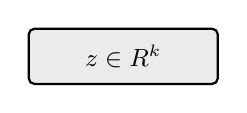
\begin{tikzpicture}
    \node[rectangle, draw=black, thick, rounded corners=2pt,
          minimum width=2.4cm, minimum height=0.7cm, inner sep=4pt,
          fill=black!8, font=\small, align=center] {$z \in \mathbb{R}^k$};
\end{tikzpicture}\\[2pt]
The bottleneck embedding. The dimensionality $k$ controls how much information passes from encoder to decoder.}

\newthought{Too few dimensions} and the encoder cannot represent the factors of variation in the data.
Reconstruction quality degrades because the embedding lacks the capacity to distinguish meaningfully different inputs.
Two inputs that differ in important ways may map to nearly identical latent vectors,
and the decoder produces a blurred average of what those embeddings could mean.


\begin{figure}
    \centering
    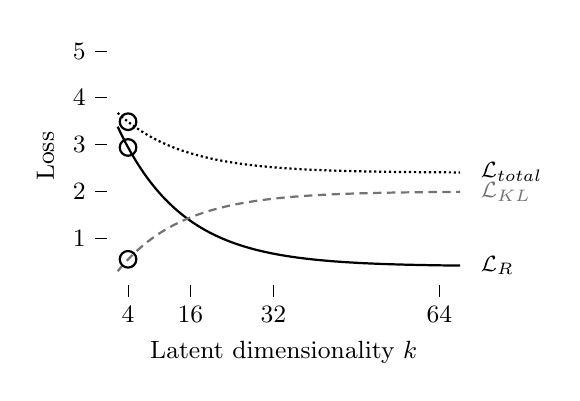
\begin{tikzpicture}[
        every node/.style={font=\small, align=center},
    ]
        \begin{axis}[
            xlabel={Latent dimensionality $k$},
            ylabel={Loss},
            xmin=0, xmax=68,
            clip=false,
            ymin=0, ymax=5.5,
            width=0.5\textwidth,
            height=0.4\textwidth,
            axis line style={draw=none},
            tick style={black, thin},
            xtick={4,16,32,64},
            ytick={1,2,3,4,5},
            xticklabel style={font=\small},
            yticklabel style={font=\small},
            tick align=outside,
            tick pos=left,
            domain=2:68,
            samples=80,
        ]
        % Reconstruction loss: decreases with k
        \addplot[black, thick] {3.5*exp(-0.08*x) + 0.4};
        \node[font=\footnotesize, anchor=west, xshift=4pt] at (axis cs:68,0.42) {$\mathcal{L}_R$};
        % KL term: increases with k (more active dims)
        \addplot[black!55, thick, densely dashed] {2.0*(1 - exp(-0.08*x))};
        \node[font=\footnotesize, black!55, anchor=west, xshift=4pt] at (axis cs:68,1.99) {$\mathcal{L}_{\text{KL}}$};
        % Total loss: L-shaped (saturates at floor)
        \addplot[black, thick, densely dotted] {1.5*exp(-0.08*x) + 2.4};
        \node[font=\footnotesize, anchor=west, xshift=4pt] at (axis cs:68,2.41) {$\mathcal{L}_{\text{total}}$};
        % Too-few regime: markers on all three curves at small k
        \addplot[only marks, mark=o, mark size=3pt, thick, black] coordinates {(4, 2.94) (4, 0.55) (4, 3.49)};
        \end{axis}
    \end{tikzpicture}
    \caption{Bottleneck too small. At $k{=}4$, reconstruction loss is large ($\mathcal{L}_R \approx 2.9$) because the few active dimensions cannot encode all factors of variation. Each active dimension carries a lot of signal, but only a handful of them are paying KL ($\mathcal{L}_{\text{KL}} \approx 0.55$). The total ($\circ$ on the dotted curve) sits high because reconstruction error dominates.}
    \label{fig:bottleneck_too_few}
    \end{figure}

\newthought{Too many dimensions} and the model faces the opposite problem.
With excess capacity, the encoder can encode each training point precisely without needing to discover shared structure.
The KL term penalises unused dimensions toward the prior, but is blended out by the reconstruction success. 
\begin{figure}
    \centering
    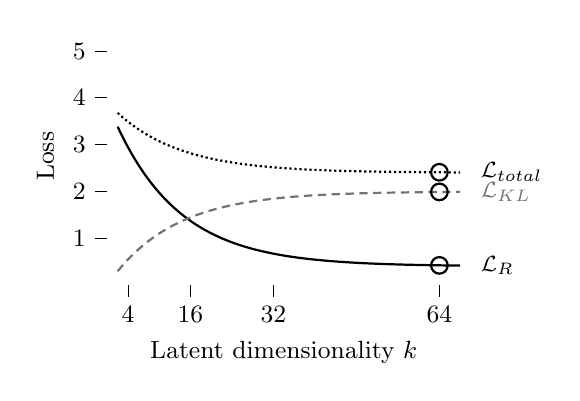
\begin{tikzpicture}[
        every node/.style={font=\small, align=center},
    ]
        \begin{axis}[
            xlabel={Latent dimensionality $k$},
            ylabel={Loss},
            xmin=0, xmax=68,
            clip=false,
            ymin=0, ymax=5.5,
            width=0.5\textwidth,
            height=0.4\textwidth,
            axis line style={draw=none},
            tick style={black, thin},
            xtick={4,16,32,64},
            ytick={1,2,3,4,5},
            xticklabel style={font=\small},
            yticklabel style={font=\small},
            tick align=outside,
            tick pos=left,
            domain=2:68,
            samples=80,
        ]
        \addplot[black, thick] {3.5*exp(-0.08*x) + 0.4};
        \node[font=\footnotesize, anchor=west, xshift=4pt] at (axis cs:68,0.42) {$\mathcal{L}_R$};
        \addplot[black!55, thick, densely dashed] {2.0*(1 - exp(-0.08*x))};
        \node[font=\footnotesize, black!55, anchor=west, xshift=4pt] at (axis cs:68,1.99) {$\mathcal{L}_{\text{KL}}$};
        \addplot[black, thick, densely dotted] {1.5*exp(-0.08*x) + 2.4};
        \node[font=\footnotesize, anchor=west, xshift=4pt] at (axis cs:68,2.41) {$\mathcal{L}_{\text{total}}$};
        % Too-many regime: markers on all three curves at large k
        \addplot[only marks, mark=o, mark size=3pt, thick, black] coordinates {(64, 0.42) (64, 1.99) (64, 2.41)};
        \end{axis}
    \end{tikzpicture}
    \caption{Bottleneck too large. At $k{=}64$, reconstruction loss has saturated near its floor ($\mathcal{L}_R \approx 0.42$) and the KL cost has saturated near its ceiling ($\mathcal{L}_{\text{KL}} \approx 1.99$): adding more dimensions changes neither term, because extra dimensions collapse to the prior and pay no KL. The total ($\circ$ on the dotted curve) sits at the plateau. The cost of $k$ too large is therefore wasted parameters and slower training, not a higher loss.}
    \label{fig:bottleneck_too_many}
\end{figure}



\newthought{The information bottleneck principle}\cite{Tishby2000} provides a theoretical lens.
The optimal embedding retains all information in $x$ that is relevant to reconstruction.
The latent dimensionality $k$ sets the ceiling on how much can be stored;
the KL weight determines how aggressively the model compresses toward that ceiling to discarding weak representations.

\begin{figure}
\centering
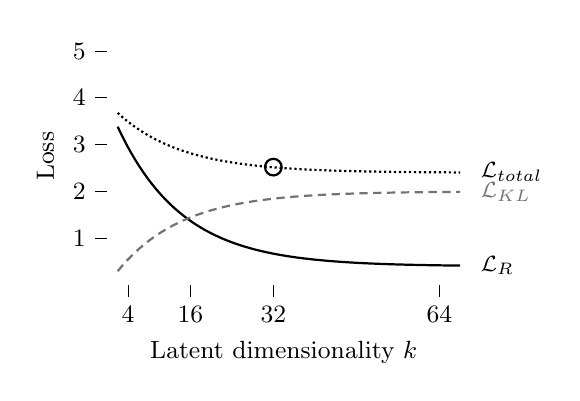
\begin{tikzpicture}[
    every node/.style={font=\small, align=center},
]
    \begin{axis}[
        xlabel={Latent dimensionality $k$},
        ylabel={Loss},
        xmin=0, xmax=68,
        clip=false,
        ymin=0, ymax=5.5,
        width=0.5\textwidth,
        height=0.4\textwidth,
        axis line style={draw=none},
        tick style={black, thin},
        xtick={4,16,32,64},
        ytick={1,2,3,4,5},
        xticklabel style={font=\small},
        yticklabel style={font=\small},
        tick align=outside,
        tick pos=left,
        domain=2:68,
        samples=80,
    ]
    % Reconstruction loss: decreases with k
    \addplot[black, thick] {3.5*exp(-0.08*x) + 0.4};
    \node[font=\footnotesize, anchor=west, xshift=4pt] at (axis cs:68,0.42) {$\mathcal{L}_R$};
    % KL term: increases with k (more active dims)
    \addplot[black!55, thick, densely dashed] {2.0*(1 - exp(-0.08*x))};
    \node[font=\footnotesize, black!55, anchor=west, xshift=4pt] at (axis cs:68,1.99) {$\mathcal{L}_{\text{KL}}$};
    % Total loss: U-shaped
    \addplot[black, thick, densely dotted] {1.5*exp(-0.08*x) + 2.4};
    \node[font=\footnotesize, anchor=west, xshift=4pt] at (axis cs:68,2.41) {$\mathcal{L}_{\text{total}}$};
    % Sweet spot: o mark at the minimum of total loss (~k=33)
    \addplot[only marks, mark=o, mark size=3pt, thick, black] coordinates {(32, 2.52)};
    \end{axis}
\end{tikzpicture}
\caption{Bottleneck sizing trade-off. Reconstruction loss (solid) falls as $k$ grows; the KL cost (dashed) rises until the data's information has been encoded, then plateaus as additional dimensions collapse to the prior. The total (dotted) is L-shaped: it drops sharply, then flattens. A good $k$ sits near the elbow ($\circ$ at $k{=}32$), where the marginal gain per added dimension has fallen below what the extra parameters and training time cost.}
\label{fig:bottleneck_tradeoff}
\end{figure}

\marginnote{\newthought{Active-unit criterion.} A latent dimension $j$ is called active if
\begin{align*}
    \mathcal{L}_{\text{KL}}\!\bigl(q(z_j|x) \,\|\, p(z_j)\bigr) &> \delta
\end{align*}
for a meaningful fraction of the training data.}

\newthought{Active units.}
Inactive dimensions have collapsed to the prior, as there is no potential reconstruction gain contributed by their information.
Monitoring the number of active units during training reveals how much of the latent capacity the model actually uses\cite{BurdaGrosseSalakhutdinov2016}.

\newthought{This reading only holds in a particular regime.}
The active-unit count is meaningful when $k$ is rather large that some dimensions could afford to drop, 
and when the reconstruction loss is competitive with the KL pull.
The diagnostic is really a measure of how many dimensions the reconstruction loss can keep alive against the KL pull.
So cross-dimension activity comparisons are needed.
\marginnote{\newthought{Rule of thumb.} For input dimensionality $d$, a reasonable starting point is $k$ on the order of $\sqrt{d}$ 
for tabular and pixel data. Text is a special case: vocabulary size makes $d$ huge ($30\text{k}+$ tokens), but semantic information for sentence-level text VAEs, start at $k{\approx}32{-}128$.}

\marginnote{\newthought{Two exceptions} where the protocol does not apply. For visualisation, set $k{=}2$ or $k{=}3$ outright and accept the fidelity loss; the goal is a readable scatter, not optimal reconstruction. For very large models, where a single training run is expensive, pick a $k$ from a comparable published architecture and skip the sweep entirely.}
\newthought{A practical protocol} for choosing $k$:
\begin{itemize}
    \item Start with a generously large $k$. Adding capacity rarely hurts validation reconstruction; it just stops helping past the elbow.
    \item Train once and read off the effective capacity. The number of active dimensions is a direct estimate of the data's information ceiling.
    \item Use validation reconstruction, not training loss, as the model-selection signal to be sensitive to overfitting.
\end{itemize}


\newthought{Beyond dimensionality,} the structure of the prior itself shapes what the latent space can express.
The standard choice $p(z) = \mathcal{N}(0, I)$ assumes the latent factors are independent and identically scaled.
When the true factors of variation have different scales, correlations, or discrete structure, a mismatched prior forces the encoder to waste capacity compensating for the mismatch.
\marginnote{\newthought{KL annealing}\cite{Bowman2016} ramps the KL weight from zero over the first $N$ epochs, letting the encoder learn useful representations before regularisation kicks in and prevents posterior collapse.}



\iffalse
\marginnote{\newthought{Free bits}\cite{Kingma2016} guarantee a minimum information rate per latent dimension by clamping each dimension's KL contribution: $\mathcal{L}_{\text{KL}}^{(j)} = \max(\lambda,\, \mathcal{L}_{\text{KL}}(q(z_j|x) \| p(z_j)))$. Dimensions below the threshold $\lambda$ incur no gradient from the KL term, preventing the regulariser from silencing them before they have learned to encode useful features.}

\newthought{Spectral normalisation}\cite{Miyato2018} constrains the Lipschitz constant of both encoder and decoder by normalising each weight matrix by its largest singular value.
This prevents the encoder from amplifying small input perturbations into large latent displacements, and prevents the decoder from producing high-frequency artefacts from smooth latent trajectories.
The result is a more stable training dynamic and a latent space where distances are more meaningful.

\marginnote{\newthought{Cyclical annealing}\cite{Fu2019} repeats the KL warm-up schedule multiple times during training rather than annealing once. Each cycle resets the KL weight to zero, allowing the encoder to reorganise its representations before the regulariser tightens again. This often yields better reconstruction and higher active-unit counts than a single linear anneal.}

\newthought{Wasserstein regularisation}\cite{Tolstikhin2018} offers an alternative to per-example KL.
Instead of requiring every individual encoding to resemble the prior, the Wasserstein Autoencoder (WAE) matches the aggregate posterior $q(z) = \mathbb{E}_{p(x)}[q(z|x)]$ to the prior using a distributional distance.
This relaxes the per-example constraint: individual encodings may look nothing like a Gaussian, as long as the overall distribution of embeddings does.
The result is a latent space that is globally well organised without forcing every input through the same narrow distributional template.
\fi





% ---------------------------------------------------------------------------
\newpage
\section{Exploring the Latent Space}\index{latent interpolation}\index{generation}

\newthought{Latent interpolation} reveals the structure that the VAE has learned.
Given two data points $x_1$ and $x_2$, encode them to $z_1 = \mu_{\theta_E}(x_1)$ and $z_2 = \mu_{\theta_E}(x_2)$, interpolate as $z_t = (1{-}t)\,z_a + t\,z_b$, and decode each $z_t$ to obtain $\hat{x}_t = \theta_D(z_t)$.
Because the latent space is regularised, the decoded path transitions smoothly between the two inputs\cite{White2016}.
Smooth interpolation is the simplest test of whether the encoder has learned a genuinely continuous feature space rather than a scattered collection of embeddings.

\begin{figure}
\centering
\begin{tikzpicture}
    \begin{axis}[
        xlabel={$z^{(1)}$},
        ylabel={$z^{(2)}$},
        xmin=-3, xmax=3,
        ymin=-3, ymax=3,
        width=0.5\textwidth,
        height=0.5\textwidth,
        axis line style={draw=none},
        tick style={black, thin},
        xtick={-2,0,2},
        ytick={-2,0,2},
        xticklabel style={font=\small},
        yticklabel style={font=\small},
        tick align=outside,
        tick pos=left,
    ]
    % Prior circles (1-sigma and 2-sigma)
    \draw[black!25, thin, dashed] (axis cs:0,0) circle[radius=1];
    \draw[black!25, thin, dashed] (axis cs:0,0) circle[radius=2];
     % Slerp waypoints with grayscale gradient z_a (light) -> z_b (dark)
    \addplot[only marks, mark=*, mark size=2pt, black!20] coordinates {(-1.06, 1.06)};
    \addplot[only marks, mark=*, mark size=2pt, black!35] coordinates {(-0.31, 1.47)};
    \addplot[only marks, mark=*, mark size=2pt, black!50] coordinates {( 0.54, 1.40)};
    \addplot[only marks, mark=*, mark size=2pt, black!65] coordinates {( 1.21, 0.88)};
    \addplot[only marks, mark=*, mark size=2pt, black!80] coordinates {( 1.50, 0.08)};
    \addplot[only marks, mark=*, mark size=2pt, black]    coordinates {( 1.30,-0.75)};
    \node[font=\small, anchor=south east] at (axis cs:-1.06, 1.06) {$z_a$};
    \node[font=\small, anchor=north west] at (axis cs: 1.30,-0.75) {$z_b$};
    \node[font=\small, black!55, anchor=south west] at (axis cs:0.54, 1.40) {$z_t$};
    \end{axis}
\end{tikzpicture}
\caption{Latent interpolation. Two inputs encode to $z_a$ and $z_b$. Linear interpolation (lerp, dashed) 
cuts through the low-density middle of the prior; in high dimensions this region is empty under $\mathcal{N}(0, I)$ 
and decoded midpoints look unnatural. Spherical linear interpolation (slerp, solid arc) follows the high-density shell 
at roughly $\|z\| \approx \sqrt{d}$, keeping every $z_t$ on-distribution. Each waypoint is decoded to produce a smooth transition.}
\label{fig:latent_interpolation}
\end{figure}

\marginnote{\newthought{Welcome to generative AI.} A trained decoder paired with a tractable prior is, in essence, a generative model: draw a vector from a Gaussian, run it through the network, and a new sample falls out the other side. Everything that followed in the field, from diffusion models to large image and video generators, builds on the same trick of learning a mapping from a simple prior to a complex data distribution.}

\newthought{Generation} is equally straightforward: sample $z \sim \mathcal{N}(0, I)$ and decode $\hat{x} = \theta_D(z)$.
The regularisation ensures that every region of the prior generates plausible data.
The same property that makes the encoder a reliable feature extractor, a latent space with no dead zones, is what makes generation possible.












% ---------------------------------------------------------------------------
\section{Brief: Feature Extraction and Transfer}\index{feature extraction}\index{backbone}\index{transfer learning}

\marginnote{\newthought{A backbone} is an encoder trained on one task, then reused as a feature extractor for another.}

\newthought{Once a VAE encoder has been trained,} the mapping $\theta_E\colon x \mapsto z$ can be detached from the decoder and reused on its own.
In practice this means freezing the encoder weights and treating its output $z$ as a fixed-length feature vector for a new, potentially unrelated task.
The frozen encoder is called a \textbf{backbone}\index{backbone}: it supplies representations; a lightweight head on top supplies predictions.

\newthought{Transfer learning}\index{transfer learning} formalises this reuse.
A model trained on a large source dataset learns general-purpose features in its hidden layers.
Those features are then transferred to a target task that may have far less labelled data.
The key insight is that early and middle layers of deep networks learn broadly useful representations (edges, textures, object parts) that are not specific to the original training objective.
The VAE encoder is one instance of this pattern: its latent embedding captures the factors of variation in the source data, and those factors are often relevant to downstream tasks as well.

\newthought{Generalisation}\index{generalisation} is the reason transfer works.
The bottleneck in an autoencoder or VAE forces the encoder to compress, and compression requires ignoring idiosyncratic noise in favour of shared structure.
A $k$-dimensional latent embedding with $k \ll d$ cannot memorise individual inputs; it must discover regularities that hold across the training distribution.
Those regularities, the semantic features, are precisely what a downstream model needs to perform well on new, unseen data.

\marginnote{\newthought{Fine-tuning vs.\ freezing.} When the target task is close to the source task, the backbone features can be used as-is (frozen). When the domains differ, fine-tuning the backbone with a small learning rate adapts the features while preserving the structure learned during pretraining.}


\newthought{The quality of transferred features depends on the source dataset.}
A backbone is only as general as the data it was trained on.
Across domains, a small number of large-scale datasets have become the standard foundations for pretraining.

\begin{table*}[ht]
\centering
\begin{tabular}{p{0.14\textwidth}p{0.10\textwidth}p{0.10\textwidth}p{0.38\textwidth}}
    \toprule
    \textbf{Dataset} & \textbf{Modality} & \textbf{Scale} & \textbf{What the backbone learns} \\
    \midrule
    ImageNet \citealt{Deng2009ImageNet} & Images & 14M images & Edges, textures, object parts, and category-level semantics. The de facto starting point for visual feature extractors. \\
    The Pile \citealt{Gao2020Pile} & Text & 825 GB text & Syntax, coreference, factual associations, and discourse structure from books, academic papers, web text, and code. \\
    LibriSpeech \citealt{Panayotov2015LibriSpeech} & Audio & 1000 h audio & Phoneme boundaries, prosody, and speaker-invariant representations from read English speech. \\
    Kinetics-700 \citealt{Carreira2022Kinetics700} & Video & 650k clips & Temporal dynamics, motion patterns, and action semantics from short video clips spanning 700 human action classes. \\
    ShapeNet \citealt{Chang2015ShapeNet} & 3D shapes & 51k models & Surface geometry, part decomposition, and pose-invariant structure from annotated CAD models across 55 object categories. \\
    LAION-5B \citealt{Schuhmann2022LAION5B} & Image + text & 5.8B pairs & Joint visual and linguistic semantics from web-crawled image-caption pairs; the foundation behind open multimodal models. \\
    CheXpert \citealt{Irvin2019CheXpert} & Medical images & 224k X-rays & Anatomical landmarks, pathology signatures, and radiological texture patterns from labelled chest radiographs. \\
    ZINC \citealt{Sterling2015ZINC} & Molecular graphs & 250k molecules & Bond topology, functional-group motifs, and drug-likeness features from curated small-molecule structures. \\
    \bottomrule
\end{tabular}
\vspace{2em}
\caption{Large-scale pretraining datasets across modalities. Each dataset provides the raw material for a backbone to learn general-purpose features that transfer to downstream tasks within (and sometimes across) its modality.}
\label{tab:pretraining_datasets}
\end{table*}

\marginnote{\newthought{Modality matters.} An ImageNet backbone transfers well to satellite imagery or medical photos, but poorly to molecular graphs or audio spectrograms. Choosing the right source dataset and modality is the first design decision in any transfer learning pipeline.}


% TODO: Knowledge Distillation is only conceptually linked to VAEs ("both compress").
% Consider moving this brief to Ch8 (Self-Supervised Learning) or Ch11 (Self-Training and Ensembles),
% where teacher-student dynamics are a more natural fit.
% ---------------------------------------------------------------------------
\section{Brief: Knowledge Distillation}\index{knowledge distillation}

\marginnote{\newthought{Distillation} transfers knowledge from a large teacher to a small student.}

\newthought{Knowledge distillation}\cite{HintonDistillation2015} compresses a large teacher model into a smaller student by training the student to match the teacher's soft output distributions rather than hard labels.

\newthought{Soft labels} are produced by scaling the teacher's logits with a temperature $T$:

\begin{align*}
    p_i^{(T)} &= \frac{\exp(z_i / T)}{\sum_j \exp(z_j / T)}
\end{align*}

Higher $T$ yields a softer distribution that reveals more about the teacher's learned structure.

\newthought{The connection to VAEs} is conceptual: both methods learn compressed representations that preserve essential information, one in the latent space, the other in the student's weights.


% ==============================================================================================
% BLOCK 3: STUDENT ACTIVATION
% ==============================================================================================

\newpage

\section{Examples \& Exercises}\index{examples}\index{exercises}

\newthought{Computing by hand} builds intuition for what the ELBO actually measures.
Step through the arithmetic slowly.

\vspace{2.5em}

% ---------------------------------------------------------------------------
% Exercise 1: ELBO derivation
% ---------------------------------------------------------------------------

\newthought{ELBO derivation.} Starting from $\log p(x) = \log \int p(x,z)\, dz$, derive the ELBO.
Work through it in four steps.

\newthought{Step 1:} introduce $q(z|x)$ by multiplying and dividing inside the integral:
\begin{align*}
    \log p(x) &= \log \int \frac{q(z|x)}{q(z|x)}\, p(x,z)\, dz \\
              &= \log\, \mathbb{E}_{q(z|x)} \left[ \frac{p(x,z)}{q(z|x)} \right]
\end{align*}

\newthought{Step 2:} apply Jensen's inequality, $\log \mathbb{E}[X] \geq \mathbb{E}[\log X]$:
\begin{align*}
    \log p(x) &\geq \mathbb{E}_{q(z|x)} \left[ \log \frac{p(x,z)}{q(z|x)} \right]
\end{align*}

Complete Steps 3 and 4 yourself: split $p(x,z) = p(x|z)\,p(z)$ and rearrange to obtain the ELBO in reconstruction + KL form.
Verify that you arrive at:
\begin{align*}
    \text{ELBO} &= \underbrace{\mathbb{E}_{q(z|x)}[\log p(x|z)]}_{\text{Reconstruction}} - \underbrace{\mathcal{L}_{\text{KL}}\!\bigl(q(z|x) \,\|\, p(z)\bigr)}_{\text{Regularisation}}
\end{align*}

\marginnote{\newthought{Why a lower bound?} Jensen's inequality introduces a gap: $\log p(x) = \text{ELBO} + \mathcal{L}_{\text{KL}}(q \| p(z|x))$. The gap is the KL divergence between the approximate and true posterior. Maximising the ELBO simultaneously improves reconstruction and pushes $q$ toward the true posterior.}


\vspace{2.5em}

% ---------------------------------------------------------------------------
% Exercise 2: KL divergence by hand
% ---------------------------------------------------------------------------

\newthought{KL divergence by hand.}
Compute $\mathcal{L}_{\text{KL}}\!\bigl(\mathcal{N}(\mu, \sigma^2) \,\|\, \mathcal{N}(0, 1)\bigr)$ for three settings.
Use the closed form $\mathcal{L}_{\text{KL}} = \tfrac{1}{2}(\mu^2 + \sigma^2 - \log \sigma^2 - 1)$.

\newthought{Setting (i):} $\mu{=}0,\, \sigma{=}1$ (the posterior matches the prior exactly).
\begin{align*}
    \mathcal{L}_{\text{KL}} &= \tfrac{1}{2}(0^2 + 1^2 - \log 1^2 - 1) \\
                  &= \tfrac{1}{2}(0 + 1 - 0 - 1) \\
                  &= 0
\end{align*}

As expected: when $q(z|x)$ exactly matches $p(z)$, the KL divergence is zero.

\newthought{Setting (ii):} $\mu{=}1,\, \sigma{=}1$ (shifted mean, same spread).
\begin{align*}
    \mathcal{L}_{\text{KL}} &= \tfrac{1}{2}(1^2 + 1^2 - \log 1^2 - 1) \\
                  &= \tfrac{1}{2}(1 + 1 - 0 - 1) \\
                  &= 0.5
\end{align*}

The encoder shifted its mean away from zero. The prior penalises this: a shifted Gaussian wastes probability mass in regions the prior considers unlikely.

\newthought{Setting (iii):} $\mu{=}0,\, \sigma{=}2$ (correct mean, too wide).
Compute this yourself, then verify:

\begin{align*}
    \mathcal{L}_{\text{KL}} &= \tfrac{1}{2}(0^2 + 2^2 - \log 2^2 - 1) \\
                  &= \tfrac{1}{2}(0 + 4 - 1.386 - 1) \\
                  &\approx 0.81
\end{align*}

The closed form splits into two independent contributions:
\begin{align*}
    \mathcal{L}_{\text{KL}} &= \underbrace{\tfrac{1}{2}\mu^2}_{\text{shift cost}} + \underbrace{\tfrac{1}{2}(\sigma^2 - \log \sigma^2 - 1)}_{\text{spread cost}}
\end{align*}

The shift cost grows quadratically with $\mu$. The spread cost is asymmetric: it grows roughly linearly as $\sigma$ exceeds 1, but blows up as $\sigma \to 0$ because of the $-\log \sigma^2$ term. This is why setting (iii) costs more than (ii).

\begin{table*}[htbp]
\centering
\begin{tabular}{p{0.10\textwidth}p{0.08\textwidth}p{0.08\textwidth}p{0.10\textwidth}p{0.35\textwidth}}
    \toprule
    \textbf{Setting} & \textbf{$\mu$} & \textbf{$\sigma$} & \textbf{$\mathcal{L}_{\text{KL}}$} & \textbf{Deviation from prior} \\
    \midrule
    (i)   & 0 & 1 & 0    & None (exact match) \\
    (ii)  & 1 & 1 & 0.50 & Shifted mean \\
    (iii) & 0 & 2 & 0.81 & Too wide \\
    \bottomrule
\end{tabular}
\vspace{2em}
\caption{KL divergence for three encoder settings. A wider posterior (iii) costs more than a shifted one (ii) because spreading probability mass away from the prior is more expensive than translating it.}
\label{tab:kl_comparison}
\end{table*}


\vspace{2.5em}

% ---------------------------------------------------------------------------
% Exercise 3: Reparameterisation
% ---------------------------------------------------------------------------

\newthought{Reparameterisation.} Why can we not directly backpropagate through $z \sim \mathcal{N}(\mu, \sigma^2)$?
Write out the reparameterised form, then verify the gradients.

\newthought{The problem:} sampling $z \sim \mathcal{N}(\mu, \sigma^2)$ is a stochastic operation with no gradient.
The parameters $\mu$ and $\sigma$ determine the distribution, but the sample itself has no differentiable relationship to them.

\newthought{The fix:} reparameterise as $z = \mu + \sigma\, \epsilon$ where $\epsilon \sim \mathcal{N}(0, 1)$.
Now $z$ is a deterministic function of $\mu$, $\sigma$, and $\epsilon$.
The randomness lives in $\epsilon$, which does not depend on the parameters.

\newthought{Numerical forward pass.} Let $\mu{=}0.5$, $\sigma{=}1.2$, and suppose $\epsilon{=}-0.3$ is sampled:
\begin{align*}
    z &= \mu + \sigma \cdot \epsilon \\
      &= 0.5 + 1.2 \times (-0.3) \\
      &= 0.5 - 0.36 \\
      &= 0.14
\end{align*}

\newthought{Verify the gradients:}
\begin{align*}
    \frac{\partial z}{\partial \mu} &= 1 \\[4pt]
    \frac{\partial z}{\partial \sigma} &= \epsilon \\
                                       &= -0.3
\end{align*}

Both are well-defined scalars.
Without reparameterisation, these gradients would not exist: backpropagation would stop at the sampling step and the encoder would receive no learning signal.


\vspace{2.5em}

% ---------------------------------------------------------------------------
% Exercise 4: ELBO evaluation by the numbers
% ---------------------------------------------------------------------------

\newthought{ELBO evaluation by the numbers.}
Combine the KL computation from the previous exercises with a concrete reconstruction to evaluate the full ELBO loss.

\newthought{Setup.} Consider a 1D VAE with encoder output $\mu{=}1,\, \sigma{=}1$ and input $x{=}3$.
After sampling and decoding, the reconstruction is $\hat{x}{=}2.7$.

\newthought{Reconstruction loss} (squared error):
\begin{align*}
    \mathcal{L}_R &= (x - \hat{x})^2 \\
                                &= (3 - 2.7)^2 \\
                                &= 0.09
\end{align*}

\newthought{KL term} (from Setting (ii) above):
\begin{align*}
    \mathcal{L}_{\text{KL}} &= 0.50
\end{align*}

\newthought{Total loss:}
\begin{align*}
    \mathcal{L} &= \mathcal{L}_R + \mathcal{L}_{\text{KL}} \\
                &= 0.09 + 0.50 \\
                &= 0.59
\end{align*}

\marginnote{\newthought{The trade-off is visible.} The reconstruction error is small (the decoder did a decent job), but the KL penalty is five times larger (the encoder strayed from the prior). A well-trained VAE balances both terms.}

Now compute the loss for a second configuration: $\mu{=}0,\, \sigma{=}1$, $x{=}3$, $\hat{x}{=}2.0$.
Which term dominates?
What does this tell you about the reconstruction-regularisation balance?

\newthought{Second configuration:}
\begin{align*}
    \mathcal{L}_R &= (3 - 2.0)^2 \\
                                &= 1.00 \\[4pt]
    \mathcal{L}_{\text{KL}} &= 0 \quad \text{(Setting (i): matches prior exactly)} \\[4pt]
    \mathcal{L} &= 1.00 + 0 \\
                &= 1.00
\end{align*}

The encoder obeys the prior perfectly ($\mathcal{L}_{\text{KL}}{=}0$), but the reconstruction suffers.
The first configuration ($\mathcal{L}{=}0.59$) achieves a better total loss by accepting some KL cost in exchange for much better reconstruction.


\vspace{2.5em}

% ---------------------------------------------------------------------------
% Exercise 5: Posterior collapse
% ---------------------------------------------------------------------------

\newthought{Posterior collapse.} Consider a VAE trained with $\beta{=}10$ in the loss $\mathcal{L} = \mathcal{L}_R + \beta \cdot \mathcal{L}_{\text{KL}}$.
After training, you observe that $\mathcal{L}_{\text{KL}} \approx 0$ for every input, and the reconstructions are blurry averages.
Diagnose what has happened.

\newthought{The diagnosis:} with $\beta{=}10$, the KL penalty is ten times more expensive than reconstruction.
The cheapest way to minimise the loss is to set $q(z|x) = p(z) = \mathcal{N}(0, I)$ for every input.
The encoder ignores $x$ entirely: $\mu \to 0$, $\sigma \to 1$.

\marginnote{\newthought{Verify.} If $\mu{=}0$ and $\sigma{=}1$ for all inputs, then $\mathcal{L}_{\text{KL}}{=}0$ (Setting (i) from the KL exercise). The KL term contributes nothing. The decoder receives the same distribution regardless of $x$, so it learns to output the mean of the training data.}

\newthought{The latent embedding carries no information.} Sampling $z \sim \mathcal{N}(0, I)$ produces the same distribution whether the input is a ``3'' or an ``8''.
The decoder cannot distinguish inputs, so it reconstructs the average digit: a blurry blob.

\newthought{Two remedies.}
\begin{itemize}
    \item \textbf{KL annealing:} start training with $\beta{=}0$ (autoencoder mode), then slowly raise $\beta$ toward 1. The encoder first learns to use the latent space, then gradually accepts the regularisation.
    \item \textbf{Free bits:} allow each latent dimension to use at least $\lambda$ nats of KL before penalising. This guarantees the encoder encodes at least some information per dimension.
\end{itemize}


\vspace{2.5em}

% ---------------------------------------------------------------------------
% Exercise 6: Coding exercise
% ---------------------------------------------------------------------------

\marginnote{\newthought{Code} will be provided as a Python notebook.
Use it as a starting point, break things, and observe what changes.}

\newthought{An MNIST digit dataset to explore.}
Train a VAE with a 2D latent space on MNIST.
Scatter-plot the latent encodings colour-coded by digit class.
Sample a grid of points from the latent space, decode them, and display the resulting digits.
Interpolate between two digits in latent space and display the decoded path.

\newthought{What to observe.}
Digit classes should form overlapping but distinguishable clusters in the 2D latent space.
The grid of decoded samples should show smooth transitions between digit types.
Increasing $\beta$ should sharpen the cluster boundaries but blur the reconstructions.


\vspace{2.5em}

% ---------------------------------------------------------------------------
\section{Self-Reflection and Recap}\index{reflection}\index{recap}

\newthought{Self-Reflection} questions to guide your thinking:
\begin{itemize}
    \item Why does the ELBO contain two terms, and what does each one enforce?
    \item What happens if you remove the KL term entirely and train with reconstruction loss alone?
    \item Why does the reparameterisation trick work, and what mathematical property of the Gaussian does it exploit?
    \item What is posterior collapse, and under what conditions does it occur?
    \item How does $\beta$-VAE encourage disentanglement, and what is sacrificed in return?
    \item Why does VQ-VAE avoid posterior collapse, and what new challenge does discrete quantisation introduce?
    \item When would you choose a conditional VAE over an unconditional one?
    \item How does the VAE latent space differ from the PCA subspace of the previous chapter, and what does the difference buy you?
\end{itemize}

\newthought{Recap} of Key Concepts:
\begin{itemize}
    \item VAEs learn probabilistic latent representations by maximising the ELBO, which trades off reconstruction fidelity against regularisation toward the prior.
    \item The reparameterisation trick enables gradient-based training by expressing the stochastic sample as a deterministic function of the parameters plus independent noise.
    \item The closed-form KL for Gaussians makes training efficient; in practice the encoder outputs $\log \sigma^2$ for numerical stability.
    \item $\beta$-VAE increases the KL weight to encourage disentanglement at the cost of reconstruction quality; VQ-VAE replaces continuous latents with discrete codes to enable autoregressive priors.
    \item Knowledge distillation is a complementary compression strategy: it transfers a teacher's soft predictions into a smaller student network.
\end{itemize}

\marginnote{\newthought{The root of VAE blindness.} A generative model can tell you what the data looks like, but not how much to trust what it says about data it has never seen.}

\newthought{A VAE trained on coffee aroma profiles} will reconstruct familiar profiles faithfully and assign them high ELBO.
A contaminated sample, one the model has never seen, will reconstruct poorly and land in a low-density region of the latent space.
The model signals that something is off, but it cannot quantify how uncertain it is, or decide what to do about it.

\newthought{Uncertainty estimation} fills this gap.
The next chapter develops tools for quantifying what a model does and does not know, distinguishing irreducible noise from reducible ignorance, and showing how uncertainty estimates enable anomaly detection, out-of-distribution flagging, and graceful degradation in deployed systems.

\marginnote{\newthought{Teaser.} A VAE assigns a reconstruction error to every input. Is a high error sufficient to declare an input anomalous, or do we need a principled measure of what the model does not know?}

\clearpage
